%*****************************************
\chapter{Future}\label{ch:future}
%*****************************************

\section{A Simple Overview}

My research on reflective thinking is leading toward a larger view of
layered human cognition.  In the future, I plan to continue to focus
on this larger architectural view.  Specifically, I am focused on the
question of how humans are capable of learning and teaching one
another to exhibit virtuous behavior.  Humans are able to learn from
each other, not just simple actions but entire systems of morality and
values. What are the factors that mitigate goal learning? What are the
differences between guilt, shame, regret?  Are these different or just
different words? Is shame fundamentally social? Guilt and shame are
common in folk psychology, but they are too poorly understood to
scientifically study the details of their specific mechanisms.

Let my working definition of virtuous behavior be the complexities of
accomplishing and maintaining social goals, which in my model are
initially learned from interactions with the physical world in the
context of parents. I am attempting to understand how different
forms of cooperative and non-cooperative behavior develop in these
situations. I am also interested in how an observant parent can
guide the development of these behaviors in children.

So, what is a simple way to begin to talk about what I mean by
``social thinking'' and ``moral thinking''? In the past, these topics
have spawned numerous approaches that are more or less representative
of my biological understanding. Some approaches have been formalized
into computational models that can be used as working scientific
theories. Recently, all of these initial approaches have been extended
and further researched so that I can calculate probability
distributions over these representations. I can now categorize these
approaches. A categorization reveals the diversity of human thought
covered by different approaches. I am interested in understanding what
types of processes are most important to describe when I approach the
extremely complicated issue of moral reasoning.

\section{Philosophy and Related Research}

\subsection{The Social Utility of Moral Reasoning}

When I approach the topic of immorality, there are many complicating
factors, so how can I simplify the reality of the situation in order
to create a model, which is necessarily not real, but which is still
useful for predicting reality? Well, I currently see many approaches
to studying different aspects of moral reasoning, such as how moral
judgements are dependent on the causal structure of how a person
understands social coersion \citep{young:2011}. I also see evidence
that engaging emotions such as ``pride'', ``embarrassment'', and
``regret'' has been shown to be correlated to specific fMRI BOLD
patterns \citep{moll:2005}. Further, lines have been drawn between
mere chauvinism for one's own social group and the more complicating
aspects of virtuous behavior that maximizes social utility
\citep{casebeer:2003}. This gives us initial evidence and
philosophical guidance to pursue better models for what I mean by
virtuous behavior.

\subsection{Current Models}

The field of machine learning has described models of goal-oriented
behavior that use a numerical utility function in order to quantify
whether or not a given goal has been accomplished. These models are
proving useful for finding the beginning of an explanation for how
models of the world are learned and what the function of specific
neurotransmitters may be in the neocortex \citep{yu:2003}. The problem
with these simple propositional goal-oriented models is that they
cannot handle the large state spaces involved in modelling social
relationships and social goals, so I need something slightly more
complicated. A popular tool for modelling situations involving people
thinking about the goals of other people is the tool of relational
representations, e.g., the modal logics of morality
\citep{horty:1994}. Augmenting goal-oriented reinforcement learning
models with the abilities of relational representations is a being
done by a relatively young field \citep{dzeroski:2001} that is proving
to be maturing very quickly.

\subsection{The Development of Social Goals}

If I am going to develop a theory of virtuous behavior, or social
goals, how do I begin to model the cooperative and non-cooperative
thought processes that would constitute working toward or against
other people? It has been shown that the neural circuits that are
involved in how someone thinks about what someone else knows are
largely distinct from the circuits involved in perceptual capabilities
\citep{bedny:2009}. There have also been distinctions shown between
the neural circuits involved in how someone thinks about what someone
else knows and executive control of actions \citep{saxe:2006}. There
is good reason to believe that the learning of social behavior is
bootstrapped from learning causal physical models \citep{perner:1991}.

\section{My Ongoing Research}

\subsubsection{A Reflective Parallel Programming Language}

I have written a programming language, called Funk2,
\citep{morgan:2009} that allows us to easily build and monitor the
execution of my model. My language allows describing systems that
reflectively trace changes to collections of knowledge by many
different parallel mental processes. Procedural reflection is a
computational technique that I have built into this language that is
useful for organizing models that monitor and control their own
execution \citep{maes:1987}. I have chosen to write my own language
because most other programming languages emphasize the idea of
abstraction barriers, which allows writing optimized code, but which
does not allow a user to access the details of an execution
environment. My language allows itself to access many of the details
of its own process execution by emphasizing ``execution simplicity''
over ``speed optimization'' in many cases. Most programming languages
are optimized for speed at the expense of the resulting complexity of
the optimized processes and also the lack of traces of reflectively
useful execution events. My language is useful for building models of
processes that monitor, control, and change other concurrently
executing processes. I see this as a very useful tool for modelling
the complex types of interactions between learning processes that are
described in the cognitive sciences. In other words, the form of
procedural reflection enabled by my language gives us a powerful
method for organizing models of parallel learning processes.

\subsubsection{A Physically Grounded Social Problem Domain}

In order to help us define a grounded problem domain, I have chosen to
focus on a rigid-body physical simulation of parents and children in
the context of basic cooking tasks in a kitchen environment. I chose
parents and children because I feel that major parts of social and
moral learning develops during early stages involving these familiar
social relationships. I chose the domain of basic kitchen cooking
tasks because this is a non-trivial social commonsense reasoning
domain that exists in some form in all human cultures.

\subsubsection{A Simple Social Reasoning Model}

\subsubsection{Physical Reactions}

My cognitive model is organized into layers. The lowest layer
represents the simplest processes of thinking, such as physical
reflexes, e.g., ``I jerk my hand away from the stove if I burn my
fingers.'' The next layer represents processes that have been practiced
successfully very often, and which one does not think about, e.g., ``My
legs go through fixed action patterns if I want to walk across the
room.''

\subsubsection{The Past, Goals, and Deliberative Thinking}

Next, at a slightly higher layer in my model, I begin to model
deliberative thinking, which allows one to use memories of the past
and imaginative memories of the future in order to make plans for
doing things that one has perhaps never done before. For example, if
one wants to rescue a cat from being caught in a tree, maybe one has
played with cats in the past as well as climbed trees, but one has
never done the two at the same time. This would be a form of
deliberative thinking, making something like a plan for a goal that
one has never exactly done before. If a plan for accomplishing a
deliberate goal is successful, perhaps this successful process could
be compiled down into a lower level layer, so that it does not need to
again be thought of deliberatively.

\subsubsection{Causal Abstractions and Reflective Thinking}

Now, I have so far only discussed the types of thought processes that
solve problems based on perceptions of problems in the physical
world. For example, the processes that reflexively jerk one's hand
from a stove, are due to corpuscles in the fingers communicating
information to neurons about burning temperatures in the skin of the
hand. Further, the learned walking process receives proprioceptive
information about the relative angles of the person's limbs, as well
as somatosensory information about the pressure on the soles of the
feet, as well as vestibular information about the accelleration forces
on the head, including gravity. Walking is a very complicated process,
but walking is primarily a physical control problem. Now, I am going
to introduce a separate perceptual stream of information that does not
describe the physical state of the body in the world. This separate
perceptual stream, refers to the interactions between the parallel
mental processes. I can distinguish between these two types of
perceptual streams, by calling one type a Physical perceptual stream
and the other I can call a Reflective perceptual stream of
information.

Now, once I have a reflective perceptual stream that represents the
reflective state of the mind, I can begin to model processes of
reflective thinking that solve problems in this reflective state
space. For example, a reflective process could remember what
deliberative processes are good for making different types of plans to
handle different types of physical problems, such as the differences
that must be considered between moving physical objects that display
agency as opposed to physical objects that do not exhibit any form of
agency. Once I have made a distinction in my model between physical
perceptions and reflective perceptions, I correlate these two streams,
which allows us to infer reflective events from physical
events.

\subsubsection{The Self/Other Distinction and Self-Reflective Thinking}

If my mental model contains knowledge of the correlations between a
physical perceptual stream and a reflective perceptual stream, then
the agent can use these correlations to predict the reflective states
of other agents based purely on their physical actions. For example,
if one agent performs a series of physical actions in order to
accomplish a goal, such as preparing a slice of buttered toast using a
knife and a loaf of bread and some butter in a kitchen, then these
actions have been correlated with this agent's reflective states,
including the current goals that the agent is pursuing. If this agent
then sees the physical world changing, and he knows that he is not
causing those changes, then he can attempt to infer the state of mind
of another agent. This type of inference process, based on the
previous correlations of physical and reflective perceptual streams,
is what I refer to as a self-reflective thought process. A
self-reflective thought process introduces the social distinction
between Self and Other reflective state knowledge that is inferred by
using the previously learned correlations between physical perceptions
and reflective perceptions. I refer to this type of self-reflective
knowledge as ``singly recursive'' reflective knowledge, or ``thinking
about what someone else is thinking about''. Sometimes this singly
recursive reflective knowledge is referred to as ``theory of mind''
knowledge in the cognitive science literature.

With self-reflective knowlege, an agent can choose to act
altruistically by helping another agent accomplish their goals or
maliciously by working against their goals. However, there is the
possibility that an agent is not always running a self-reflective
process that pays attention to another agent's physical actions in
order to infer what their goals might be. In many cases, such as in
my simulation of parents and children in a kitchen, some agents might
focus single-mindedly on a novel task without thinking about what the
goals of surrounding agents might be. This type of model allows for an
agent that works against the goals of another agent without knowing
the goals of the other agent. One might argue that this type of
situation where one agent clobbers the goals of another agent is due
to a form of self-reflective laziness and not due to malicious
intentions.

\subsubsection{Guilt, Pride, and Self-Conscious Thinking}

Because I am interested in modelling how children learn from parents
as well as how parents guide a child's cooperative behavior, I need
to extend my model slightly in order to allow for modelling what one
agent thinks about what another agent thinks about her. This form of
double reflective recursion is what I refer to as a self-conscious
knowledge and the problems that are represented in this type of
knowledge are handled by what I call self-conscious thought
processes. For example, a little boy may be cooking something in the
kitchen and he may carelessly work against the goals of his sister;
this situation may be recognized by an onlooking parent, and the
parent may inform the boy of a self-reflective mistake he has made:
``Ralph, your sister was going to use some of that butter that you just
finished.'' The little boy, Ralph in this case, thinks that his mother
thinks that he made a self-reflective mistake. I hypothesize that
modelling this form of double reflective recursion in conjunction with
respectful social relationships may be useful for understanding
emotions such as guilt and pride. I have focused my model of
children learning to cooperate in the context of parents on this sort
of self-conscious learning feedback.

\subsection{A Six Layer Organization of My Theory}

My layered reflective model of mind is inspired by Minsky's Model-6
Emotion Machine theory of how humans perform commonsense human
thinking \citep{minsky:2006}.

\begin{itemize}
\item{Self-Conscious Thinking: processes that manipulate doubly recursive reflective representations.}
\item{Self-Reflective Thinking: processes that manipulate singly recursive reflective representations.}
\item{Reflective Thinking: processes that manipulate representations about one's own mind.}
\item{Deliberative Thinking: processes that manipulate representations of the physical world.}
\item{Learned Reactive Thinking: processes that have been learned and chunked for efficient execution.}
\item{Built-In Reactive Thinking: processes that are given as the simplest and lowest-level aspects of the mental model.}
\end{itemize}

In summary, the control structure in my model can be thought of simply
as being roughly organized into six layers of control.  The bottom
layer represents the physical reactive interface to the physical
world. Both perception and action are inputs and outputs from this
layer, respectively. Then, at each subsequently higher layer
information from below and above are processed as I have described in
the previous sections, leading to changes in self-reflective processes
caused by self-conscious learning as my highest level example.




\section{Panalogy Architecture}



\subsection{Recursive Loops and Infinite Recursive Tracing Descent}

If the focus on the tracing is controlled carefully, these potential
loops can be avoided.  How to detect and control these potential loops
is an interesting area of future automatic debugging research in
reflective control.

\subsection{Potential Future Uses for Low-Level Tracing}

Lower level objects maybe be interesting to focus on for research in
automatic abstraction and simulation of system components.  Optimizing
compilers could benefit from this area of future research.  E.g.
focusing on the CPU object could help to develop better run-time
register allocation models.

\subsection{Why Should You Use This Radically New Language?}

Because the language is very similar to Lisp, it has proven to be easy
for both expert and novice programmers to learn.  This has been my
experience with the four undergraduates that have worked within the
language, who learned it quickly, started writing their own macros to
facilitate their style, and one even made additions to the core
algorithms.

\section{Agent Speech Acts}

At any given point in time, each agent is pursuing a different variety
of goals.  Each agent executes actions in order to accomplish
collections of these goals.  I treat language communication as an
additional physical action that the agent can choose to perform in
order to accomplish its goals.

\section{Modelling Noise in Agent Communication}

\begin{figure}[bth]
  \center
  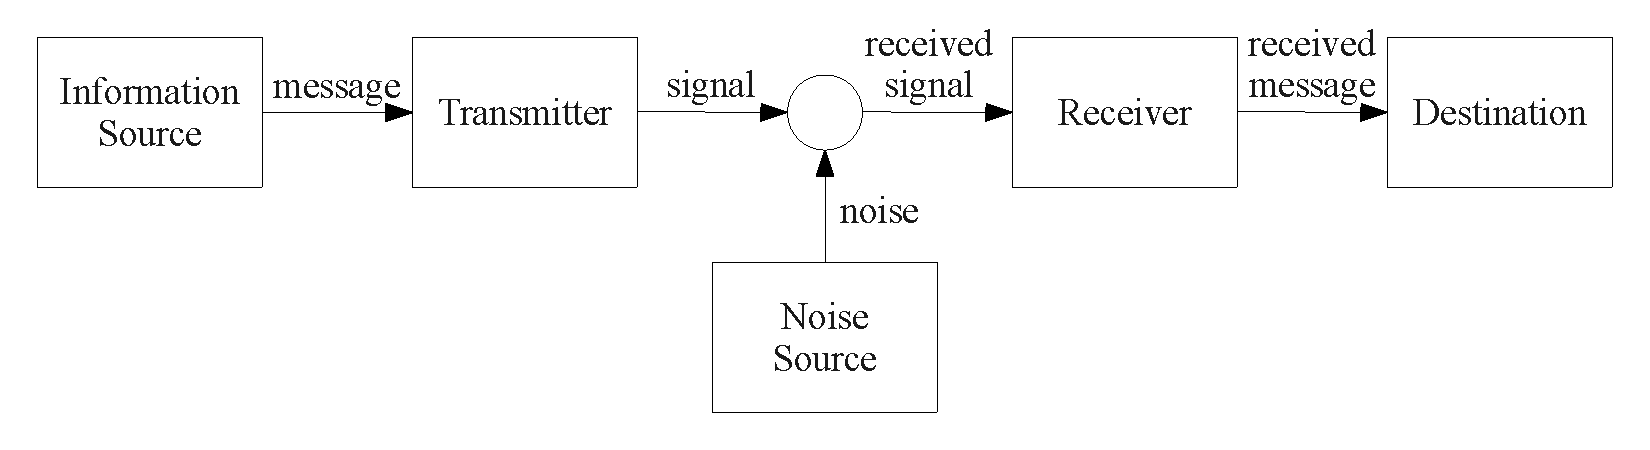
\includegraphics[width=10cm]{gfx/communication_theory}
  \caption[A mathematical theory of communication]{A mathamtical
    theory of communication~\citep{shannon:1959}.}
  \label{fig:communication_theory}
\end{figure}

My cognitive theory makes no statements as to the presence of noise
in communication channels between agents and the environment.
Communication between agents and the environment in my implementation
occurs across a noiseless communication channel.  It is theoretically
possible to include a theory of noisy communication channels between
agents and the environment.  For example, Shannon's mathmematical
theory of communication~\citep{shannon:1959} could be applied as an
elaboration to any of the information pathways in my basic theory.


% horvat:
%
%   you consider the perception independent from the agent, i.e. many
%   agents can have the very same perception... against Schopenhauer:
%   "one can thus no longer separate the perceiver from the perception"
%   (The World as Will and Presentation) -> future work ;-)
%

\section{Applications to Education and Mental Health}

An exciting new field is growing to include applications of cognitive
theories of mind to both educational and clinical mental health
domains.  For example, \cite{mahncke:2006} have reported results of
improved cognitive function by using an automated computer cognitive
training program targeting age-related cognitive decline.



